\subsection{Computer Vision}

Computer vision is an interdisciplinary field that  enables computers to interpret images just as what we human can do. Its goal is about automatic extraction, analysis, and understanding of the information from images \cite{BMVA}. There are a huge variety of ways to process images and a marvellous diversity of applications in this board field, ranging from replicating human visual abilities to creating nonhuman visual capabilities \cite{Goodfellow-et-al-2016}. Some real-world applications include object recognition or detection, 3D model building, motion capture, etc \cite{szeliski2011computer}.

Despite all the progress achieved, computer vision systems are still so underdeveloped that they can't match the visual ability of a 5 year-old child. Vision is natural and effortless for humans but factitious and demanding for computers \cite{parallel}. The difficulty in part results from that vision is a inverse problem where we attempt to recover the unknowns, \eg shape and illumination,  based on insufficient information of their causes, \eg models \cite{szeliski2011computer}.  Therefore, it is hard to  conclude the clear rules that can help get a solution explicitly, especially for complex problems, \eg 3D object detection. But currently, Deep Learning seems to find a way out and pushes a big step forward.

Next in this section, we introduce some basic knowledge in computer vision related to our approach.

\subsubsection{Image Formation}

Imaging systems or cameras are some devices that allow the projection of light from 3D points to some 2D medium that records the light pattern. Figure \ref{figure:camera} (a) shows a pinhole imaging model which is able to capture the light pattern, the inverted candle image, by allowing a very tiny cone of rays issued  at every point of the source, the real candle,  to project on the image plane. This is called pinhole perspective projection which is primitive but provides an acceptable approximation of the imaging process \cite{Forsyth:2002:CVM:580035}. 

The projection equation can be derived from Figure \ref{figure:camera} (b), where $ (O, i, j, k) $ is the pinhole camera coordinate system and the origin $O$ is at the pinhole,  $p=(u, v, d)^T$ is a point in image, and   $P=(x, y, z)^T$ is a point denotes the source. As light travels straight in the same medium, $p, O$ and $P$ are collinear, and therefore we can deduce  

\begin{equation}
\label{eq1}
	\begin{cases}
	u = d\frac{x}{z}, & \\    
	v = d\frac{y}{z}   
	\end{cases}
\end{equation}

Modern cameras are built on lenses that can gather more light to make the image more bright while maintaining its sharpness. But the imaging process is very similar to the pinhole camera. Lenses can also introduce some aberrations, \eg spherical aberration, radial distortion, and chromatic aberration \cite{Forsyth:2002:CVM:580035}. Therefore, correction is necessary.

\begin{figure}[h]		
	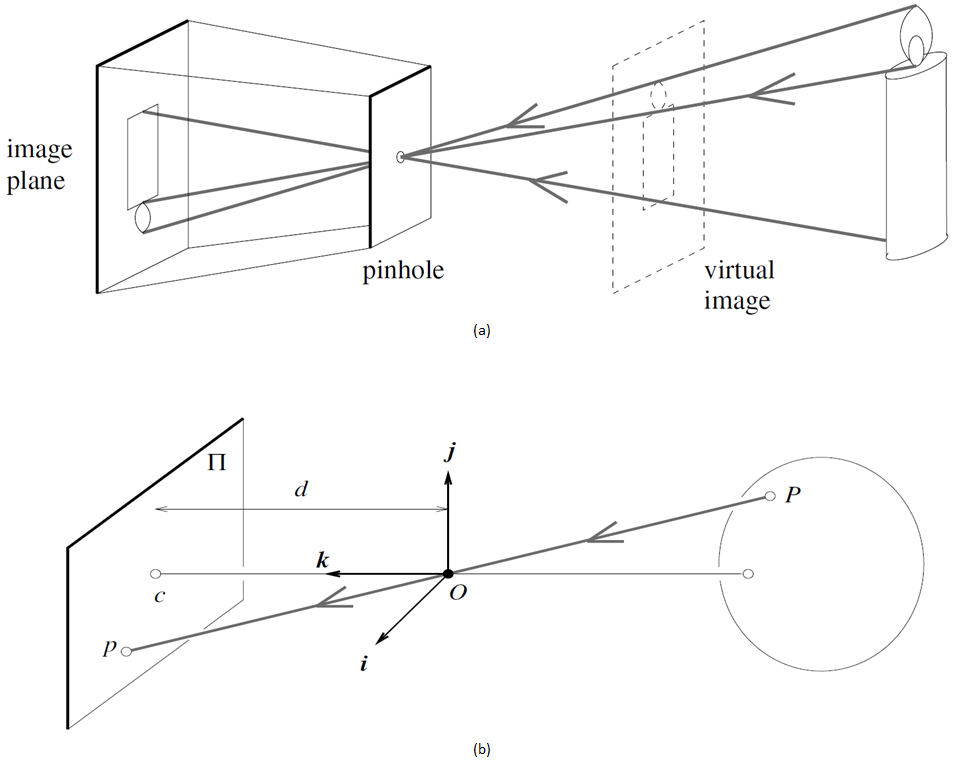
\includegraphics[width=1\textwidth]{camera.png}
	\caption{(a). the pinhole imaging model; (b). geometric model for perspective projection. \cite{Forsyth:2002:CVM:580035}}
	\centering
	\label{figure:camera}
\end{figure}

\subsubsection{Intrinsic and Extrinsic Parameters}
\label{projection}

To project a 3D point in the world coordinate system, first we have to transform this point to the camera coordinate system and then transform it to the image plane. The first transformation depends on the extrinsic parameters while the second rely on intrinsic parameters.

\textbf{Intrinsic parameters} include the focal length $f$ just like the $d$ in Figure \ref{figure:camera} (b), the image coordinates origin $(u_0, v_0)$, and the skewed angle $\theta$ of two image axes. Coordinates in image plane are usually expressed in pixel which can be square or rectangular. So let's assume $\alpha$ and $\beta$ are the value expressed $f$ with horizontal and vertical pixel-meter scales. Therefore, we can finally transform Eq. \ref{eq1} into 
\begin{equation}
\label{eq2}
	\begin{cases}
	u = \alpha \frac{x}{z} - \alpha \cot\theta + u_0, & \\    
	v = \frac{\beta}{\sin\theta} \frac{y}{z} + v_0
	\end{cases}
\end{equation}

When it is written in matrix form as Eq \ref{eq3}, the $3\times3$ matrix $K$ is the intrinsic matrix of the camerac. Note that $P$ is expressed in camera coordinate system and $p$ is in image coordinate system.

\begin{equation}
\label{eq3}
p = K P \Leftrightarrow \frac{1}{z}
\bigl(\begin{smallmatrix}
u\\  v \\1
\end{smallmatrix}\bigr) 
= 
\begin{pmatrix}
\alpha & -\alpha \cot\theta & x_0\\ 0 & \frac{\beta}{\sin\theta}  & y_0\\  0 &0  &1 
\end{pmatrix}
\begin{pmatrix} 
x\\  y\\  z
\end{pmatrix}
\end{equation}

\textbf{Extrinsic parameters} defines a rigid transformation from world coordinate system to camera frame. A rigid transformation has six degree of freedom, including three Euler angles expressed in a $3\time3$ rotation matrix $R$ and three translation components along each axis expressed in a $1\times3$ translation vector $t$. A point expressed in homogeneous coordinates is $P=(x, y, z, 1)^T$. Homogeneous coordinates can simplify various geometric transformations into matrix multiplication \cite{Forsyth:2002:CVM:580035}.  Therefore, this rigid transformation expressed in homogeneous coordinates is 
\begin{equation}
\label{eq4}
P^{C} = T_W^C P^W, where ~~T_W^C = 
\begin{pmatrix}
	R & t\\ 
	0^T& 1
\end{pmatrix}
\end{equation}
$P^{C}$ and $P^W$ are coordinates of the same point expressed in world coordinate system and camera coordinate system respectively. $T_W^C$ is the extrinsic matrix of the camera.

To put it all together, the projection equation in homogeneous coordinates is 
\begin{equation}
\label{eq5}
p = \frac{1}{z} M P^W = \frac{1}{z} K
\begin{pmatrix}
R & t\\ 
0^T& 1
\end{pmatrix} P^W
\end{equation}
where $M$ is the \textbf{perspective projection matrix}.